\title{Lab3: Programación bajo plataformas abiertas}
%%%%%%%%%%%%%%%%%%%%%%%%%%%%%%%%%
%%% Laboratory report v2
%%% Universidad de Costa Rica
%%% Ricardo Román-Brenes
%%% ricardo.roman@ucr.ac.cr
%%%%%%%%%%%%%%%%%%%%%%%%%%%%%%%%%
\documentclass[11pt]{article}

% Document config
\usepackage[letterpaper, margin=1in]{geometry}
\usepackage[spanish]{babel}
\usepackage[utf8]{inputenc}
\usepackage{tikz}
\usepackage{hyperref}
\usepackage{color}
\usepackage{xcolor}
\usepackage{float}
\usepackage{tcolorbox}
\usepackage{pdfpages}

% Color definitions
\definecolor{darkblue}{rgb}{0 , 0.054 , 0.196}
\definecolor{mygreen}{rgb}{0,0.6,0}
\definecolor{mygray}{rgb}{0.8,0.8,0.8}
\definecolor{codeBG}{rgb}{0.9, 0.97, 0.9}
\definecolor{mymauve}{rgb}{0.58,0,0.82}

\addto\captionsspanish{% Replace "english" with the language you use
  \renewcommand{\contentsname}%
    {Tabla de contenidos}%
}



% \title{
% {
%     \begin{tikzpicture}[overlay, remember picture]
%         \node[anchor=north west, %anchor is upper left corner of the graphic
%             xshift=3cm, %shifting around
%             yshift=-4cm] 
%             at (current page.north west) %left upper corner of the page
%         {\includegraphics[height=1.3cm]{img/logoEIE.png}}; 
%     \end{tikzpicture}
%     \begin{tikzpicture}[overlay, remember picture]
%         \node[anchor=north east, %anchor is upper left corner of the graphic
%             xshift=-3cm, %shifting around
%             yshift=-4cm] 
%             at (current page.north east) %left upper corner of the page
%         {\includegraphics[height=1.3cm]{img/logoUCR.png}}; 
%     \end{tikzpicture}
%     \Large 
%         \textbf{Universidad de Costa Rica}\\
%         Facultad de Ingeniería\\
%         Escuela de Ingeniería Eléctrica\\~\\
%         \texttt{IE-0117} Programación Bajo Plataformas Abiertas
%     }
%     ~\\~\\
%     {\LARGE Laboratorio 0: Instalando GNU/Linux}
% }
% \author{M. Sc. Ricardo Román Brenes - \texttt{ricardo.roman@ucr.ac.cr}}
% \date{I-2018}

\begin{document}
% \maketitle

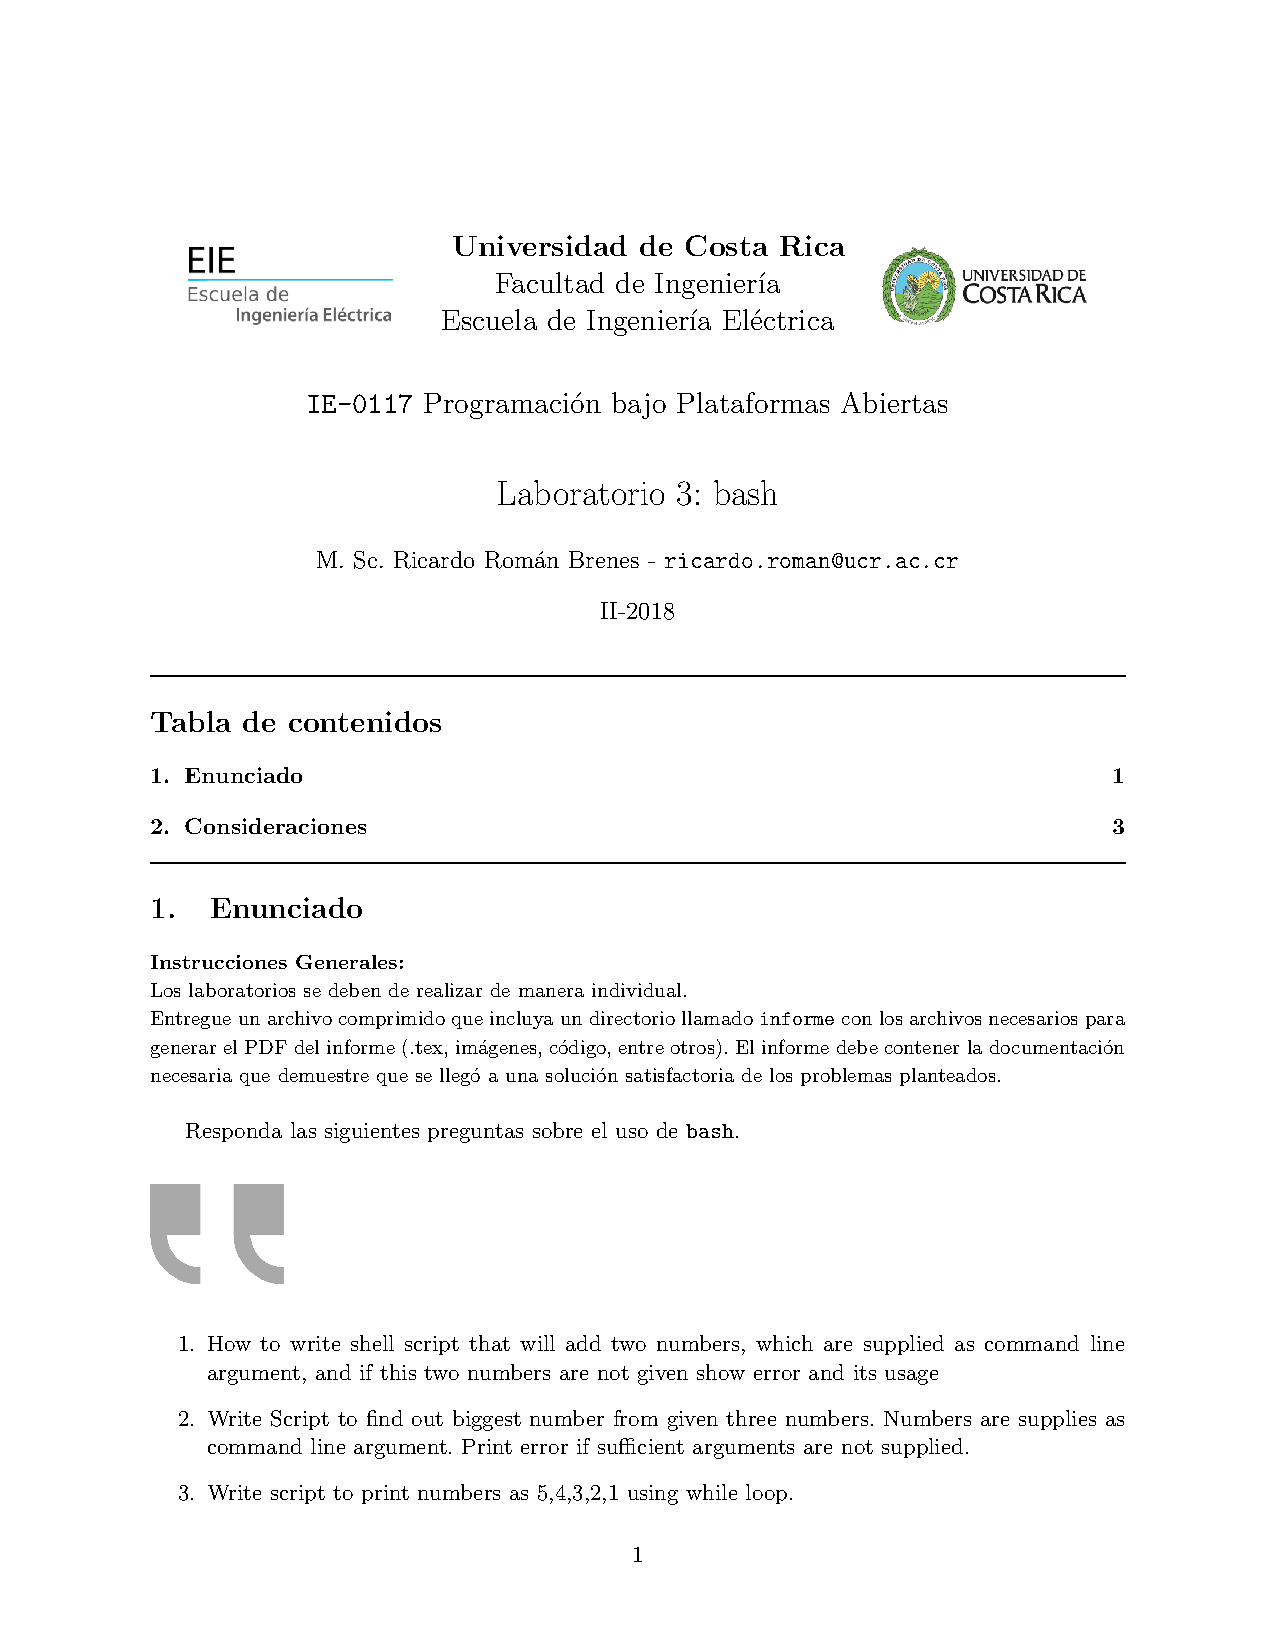
\includepdf[pages=-]{pdf/Lab3}
\tableofcontents
\hspace{5mm}
\hrule
\hrule



\subsection{Desarrollo}

Se utilizó el editor de texto ATOM para generar los scripts

\begin{enumerate}
\item Anadiendo dos números enviados desde la línea de comandos

\begin{figure}[H]
  \centering
    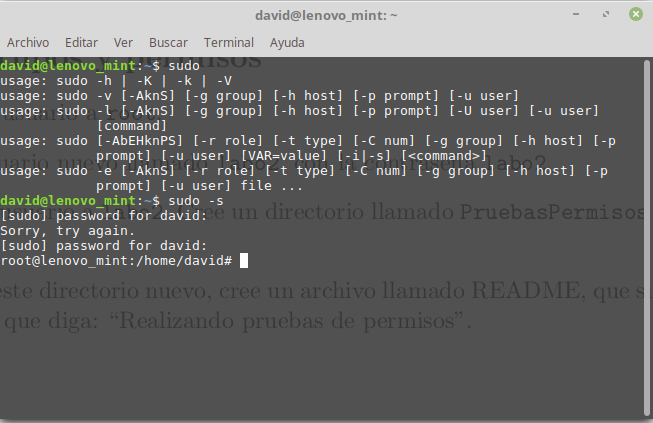
\includegraphics[width=0.7\textwidth]{img/1}
  \caption{Usuario root.}
\end{figure}

\item  Para crear un usuario nuevo llamado labo2, con la contraseña labo2 se utilizan el comando adduser y este solicita toda la información necesaria para crearlo, incluyendo la contraseña
\begin{figure}[H]
  \centering
    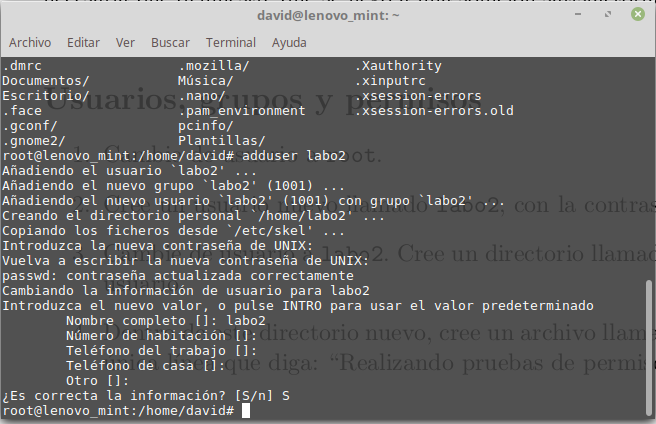
\includegraphics[width=0.7\textwidth]{img/2}
  \caption{Creación de usuario.}
 
\end{figure}

\item Se procede a cambiar de usuario a labo2 con el comando su.
\begin{figure}[H]
  \centering
    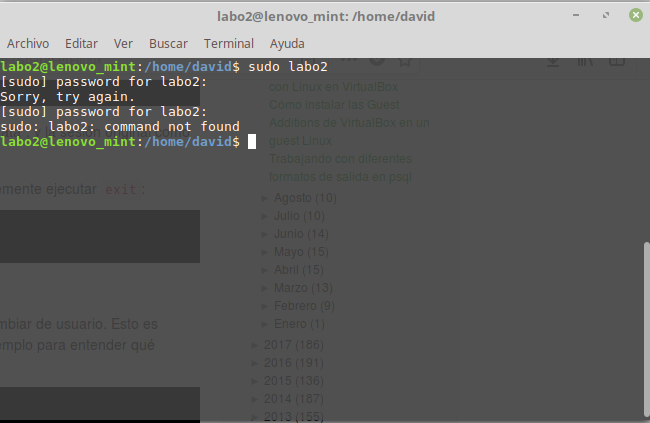
\includegraphics[width=0.7\textwidth]{img/3}
  \caption{Direccionamiento relativo.}
 
\end{figure}

\item  Una vez en labo2 se crea un directorio llamado PruebasPermisos con el comando mkdir.
\begin{figure}[H]
  \centering
    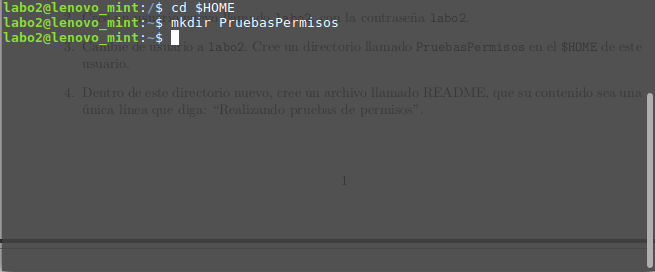
\includegraphics[width=0.7\textwidth]{img/4}
  \caption{Creación de un directorio PruebasPermisos.}
 
\end{figure}

\item Se procede a crear un Readme con el comando touch y con el editor nano se procede a escribir la línea: Realizando pruebas de permisos.
\begin{figure}[H]
  \centering
    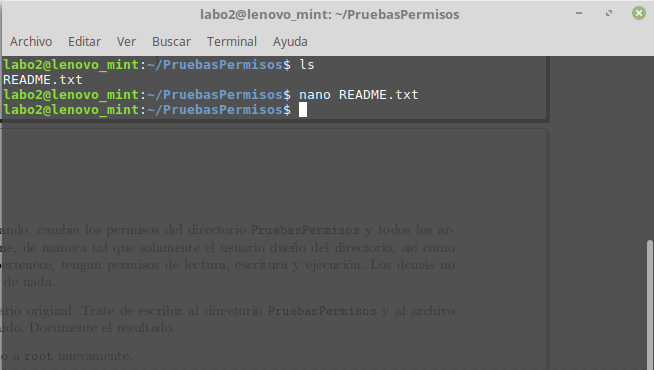
\includegraphics[width=0.7\textwidth]{img/5}
  \caption{Creación de un Readme en el usuario labo2.}
 
\end{figure}

\item Se cambian los permisos del directorio PruebasPermisos y todos los archivos que contiene utilizando el comando chmod.
\begin{figure}[H]
  \centering
    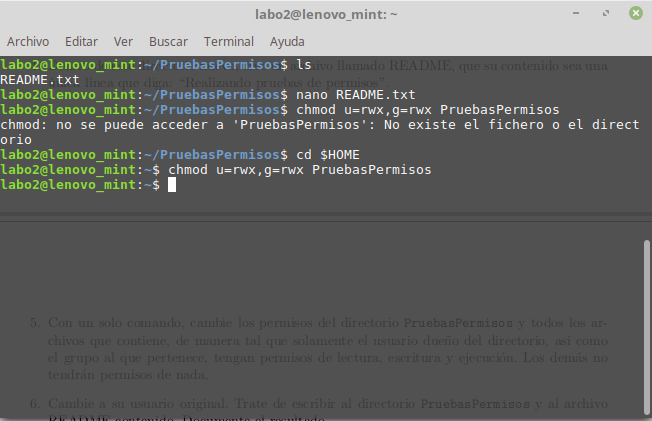
\includegraphics[width=0.7\textwidth]{img/6}
  \caption{\$HOME.}
 
\end{figure}

\item Para el cambio al usuario original se utiliza exit, y en el momento en el que se intenta escribir al directorio PruebasPermisos y el archivo README contenido en el directorio se genera un error porque el archivo y el directorio no existen en este usuario. 
\begin{figure}[H]
  \centering
    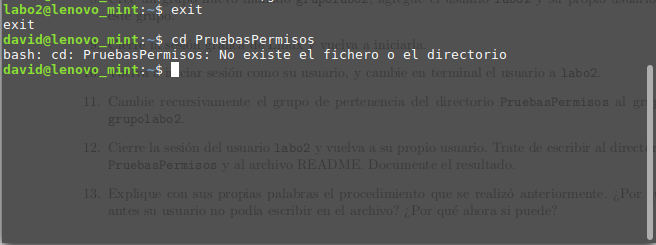
\includegraphics[width=0.7\textwidth]{img/7}
  \caption{Escritura al directorio desde el usuario original.}
 
\end{figure}

\item Se cambia a usuario root de nuevo mediante el comando sudo -s
\begin{figure}[H]
  \centering
    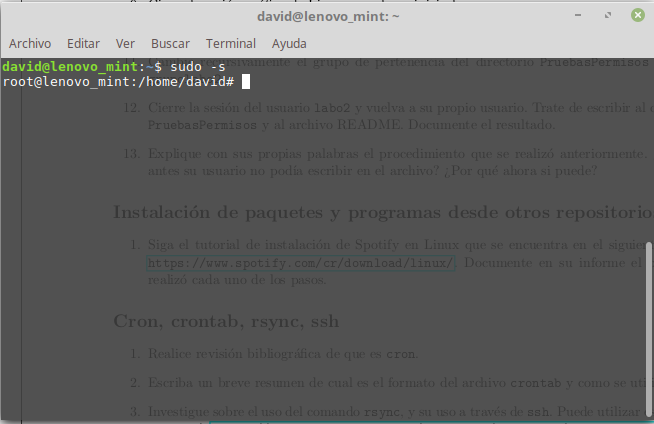
\includegraphics[width=0.7\textwidth]{img/8}
  \caption{}
 
\end{figure}

\item Se crea un nuevo grupo llamado grupolabo2 y se procede a agregar el usuario labo2 y mi propio usuario al grupo creado nuevamente mediante el comando usermod.

\begin{figure}[H]
  \centering
    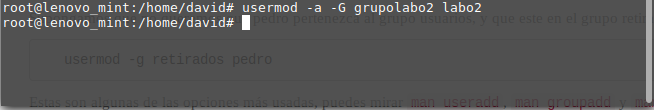
\includegraphics[width=0.7\textwidth]{img/9}
  \caption{Cambio de grupo de usuarios.}
\end{figure}

\begin{figure}[H]
  \centering
    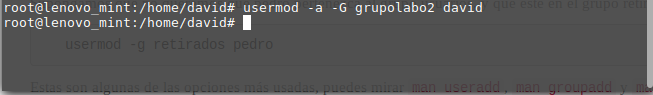
\includegraphics[width=0.7\textwidth]{img/10}
  \caption{Cambio de grupo de usuarios.}
\end{figure}

\item En este paso se procede a cerrar la sesión gráfica.

\item Se procede a volver a iniciar sesión y cambiar el usuario a labo2.
\begin{figure}[H]
  \centering
    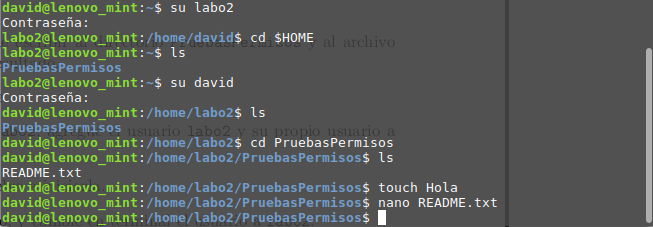
\includegraphics[width=0.7\textwidth]{img/13}
  \caption{Inicio de sesión nuevamente.}
\end{figure}

\item Se procede a cambiar recursivamente el grupo de pertenencia del directorio PruebasPermisos al grupo grupolabo2, esto quiere decir que todos los subdirectorios pasan a formar parte del grupo grupolabo2.

\begin{figure}[H]
  \centering
    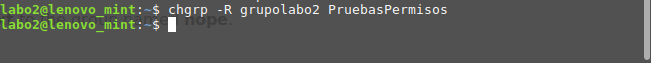
\includegraphics[width=0.7\textwidth]{img/25}
  \caption{Cambio de grupo de manera recursiva.}
 \end{figure} 

\item Se procede a cambiar al usuario original y ahora sí es posible escribir al directorio PruebasPermisos y al archivo README.


\item En el paso anterior lo que sucede es que ya se puede acceder debido a que se el usuario personal y los archivos que se pretenden accesar están en el mismo grupo de permisos, por lo que ahora sí se tiene permisos de lectura y escritura y anteriormente no.


 
 \item Instalación de paquetes y programas desde otros repositorios. Se procedió a instalar Spotify, siguiendo los pasos del link de descarga para linux, basicamente sudo apt install spotify.
 
 \begin{figure}[H]
  \centering
    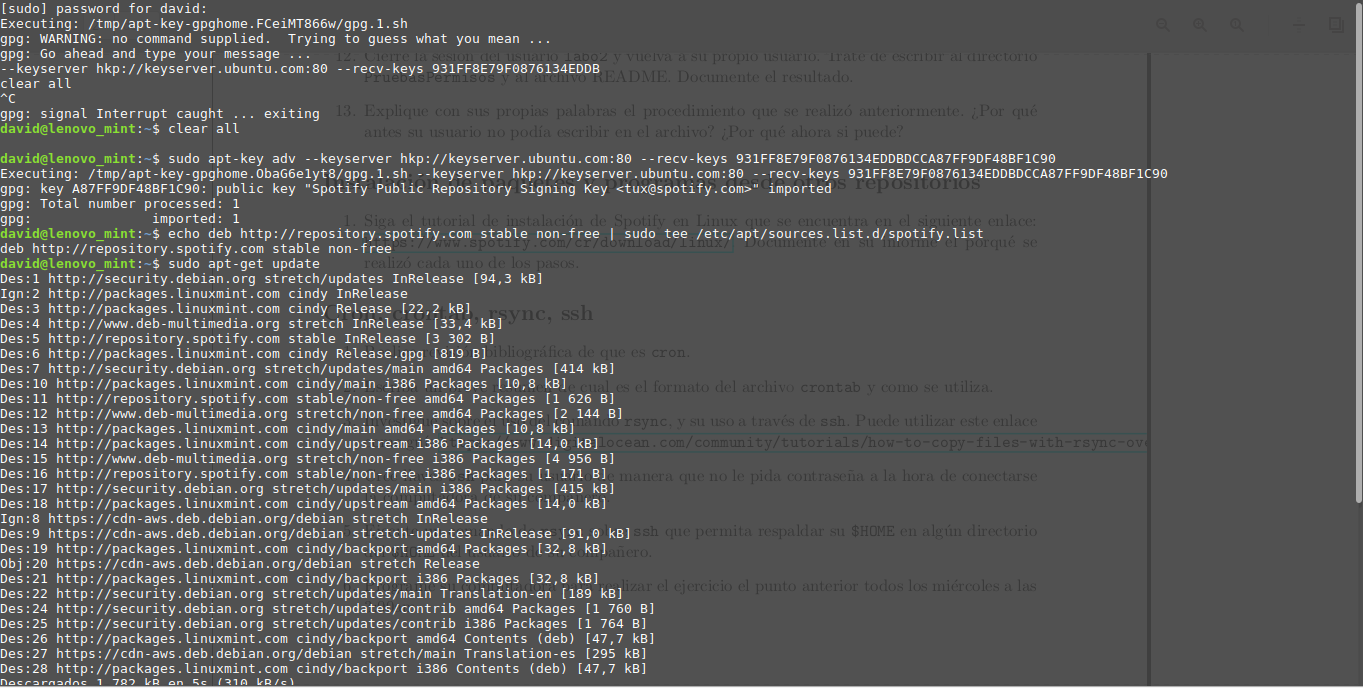
\includegraphics[width=0.7\textwidth]{img/28}
  \caption{Instalación de spotify}
\end{figure}

\end{enumerate}

 
 \subsection{Uso de Cron, crontab, rsync, ssh}

\begin{enumerate}

 \item Realizando una revisión bibliográfica de Cron se entiende que es un proceso que ejecuta un proceso previamente definido y configurado en un momento específico del horario del sistema definido por el usuario de manera automatizada.\cite{Cron}
 

 
 \item El formato del archivo crontab es de la siguiente forma:
 
 Se utiliza siguiendo el siguiente comando:
 
 



 \item Se hizo lectura del comando rsync y su uso a través de ssh utilizando el enlace de la guía, obteniendo como resultado la comprensión básica del comando rsync y cómo se pueden crear llaves para compartir información sin necesidad de ssh.
 
 \item Para la creación de llaves se siguieron los comandos de la guía suministrada, con estos pasos se crea la llave para que el compañero pueda hacer uso de ella y utilizarla para transferir archivos. Cabe destacar que no hay que incluir contraseñas en el paso de creación de la llave.
 
 \item Se ejecuta el comando de rsync que me permite copiar mis archivos al directorio de mi compañero.
 
\begin{figure}[H]
  \centering
    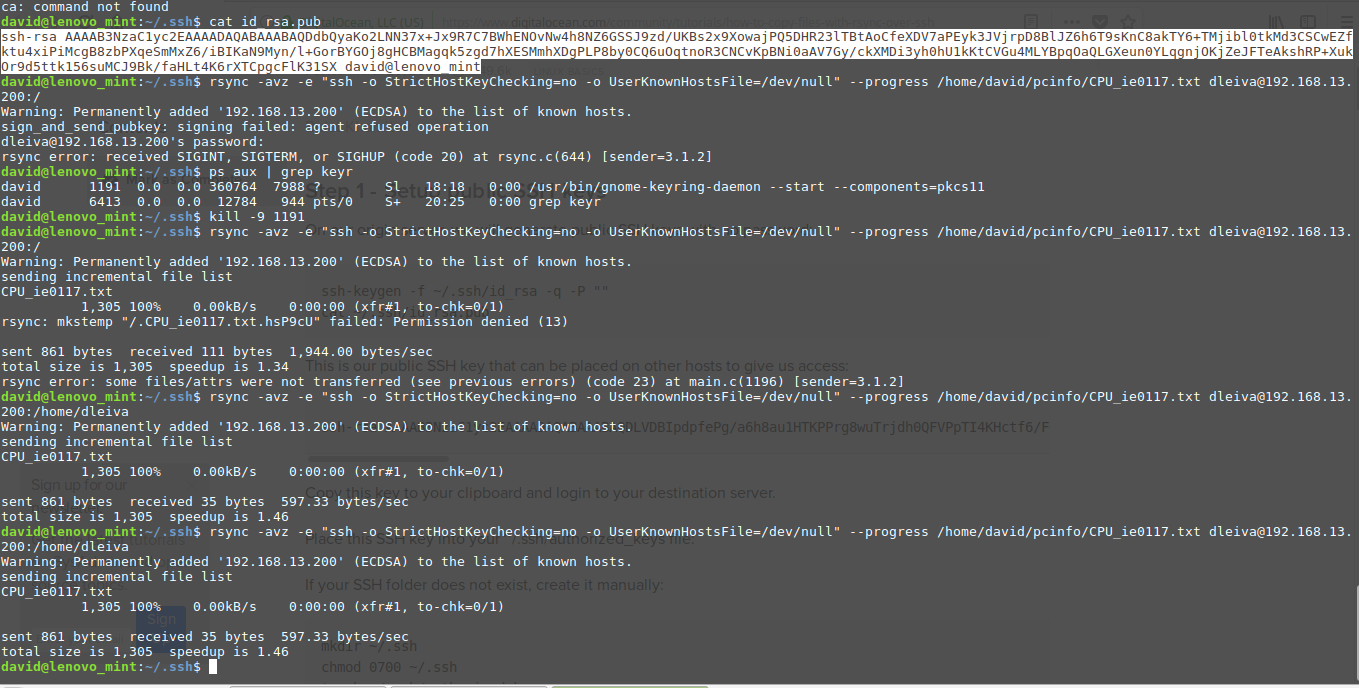
\includegraphics[width=0.7\textwidth]{img/29}
  \caption{Uso de rsync para acceso a directorios de un compañero.}
\end{figure}


\item Se utiliza el comando crontab para programar en mi computadora el ejercicio anterior todos los miércoles a las 3:00am.

\end{enumerate}

\begin{figure}[H]
  \centering
    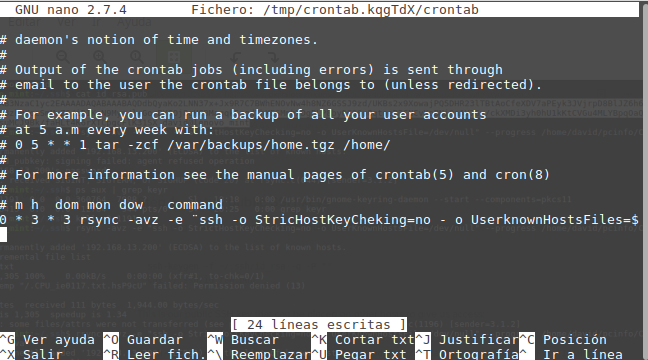
\includegraphics[width=0.7\textwidth]{img/33}
  \caption{Configuración de tarea programada.}
\end{figure}



\subsection{Intalación de programas desde código fuente}

\begin{enumerate}

 \item Se visitó el enlace proporcionado en la guía sobre ffmpeg.
 
 \item Se procedió a descargar el fichero ffmpeg.tar.bz2
 
 \item Para intalar el programa se descomprimió el archivo descargado, se revisó el arhivo install y con este se logró instalar el programa.

\begin{figure}[H]
  \centering
    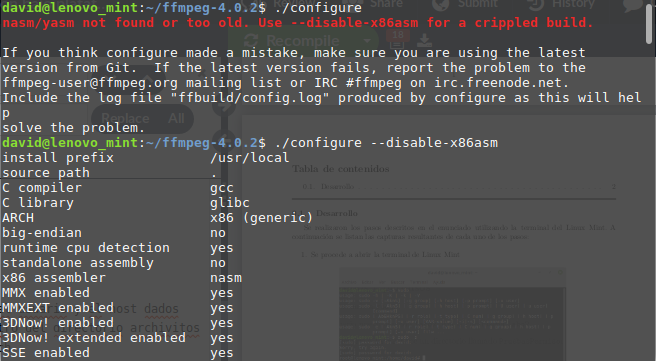
\includegraphics[width=0.7\textwidth]{img/30}
  \caption{Instalación desde código fuente.}
\end{figure}

\begin{figure}[H]
  \centering
    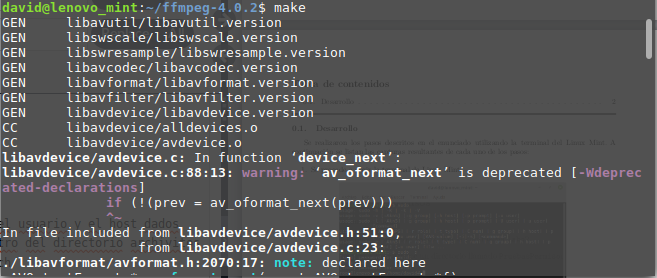
\includegraphics[width=0.7\textwidth]{img/31}
  \caption{Instalación desde código fuente.}
\end{figure}

\begin{figure}[H]
  \centering
    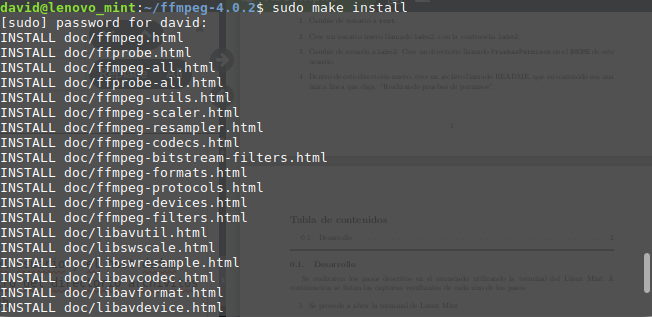
\includegraphics[width=0.7\textwidth]{img/32}
  \caption{Instalación desde código fuente.}
\end{figure}

\end{enumerate}

\newpage
\bibliographystyle{plain}
\bibliography{2.bibliography}

\end{document}
